\chapter{绪论}

\section{机器学习与正则化}

机器学习是人工智能的一个子领域,它着眼于设计和开发能自动从数据中生成出模型的算法。机器学习又
被细分为监督学习、无监督学习以及半监督学习、增强学习等类别,但是它们的思路都是相似的,亦即对
问题进行建模,并寻找一个最适合给定约束条件的函数或模型,通常约束条件直接来自于训练数据。如果
训练数据的数量足够多,我们通常能得到比较好的结果,然而大多数时候训练数据总是不够的,此时我们
通常会遇到有很多(甚至无穷多个)满足约束条件的解的情况,并且大部分这样的解在未知数据上的表现
非常差。换句话说,这样的问题是数值不稳定的,或者说泛化性能很差。

一种解决办法就是正则化(Regularization),亦即对可能解空间进行限制,这种技术最初由
Tikhonov 和 Arsenin \cite{tikhomirov1960dsf} 提出,用于解决矩阵求逆的问题,并且后
来被成功地应用到机器学习中来。许多机器学习的算法(例如支持向量机)都可以看成是某
种形式的正则化。简单来说,正则化可以看作是关于待解决问题的某种先验的知识,例如,在
脊回归(Ridge Reguression)中的正则化可以看作是将参数的先验分布定为高斯分布的结果,
而流形正则化(Manifold Regularization)\cite{On-Manifold-Regularization} 则是编码了
数据点都分布在一个低维流形上这样一个先验假设。

虽然正则化如今已经成为机器学习中广泛使用的一种技术,大多数情况人们都只考虑了问题在空间上的
属性。当我们遇到随时间变化的数据(例如,动态网页、博客内容或者股票价格等)时,一个很自然的
想法就是要保证数据在时间上的平滑性,这样的假设通常能帮助我们得到更健壮的解。

\section{时空正则化与视频压缩}

\begin{figure*}
\center{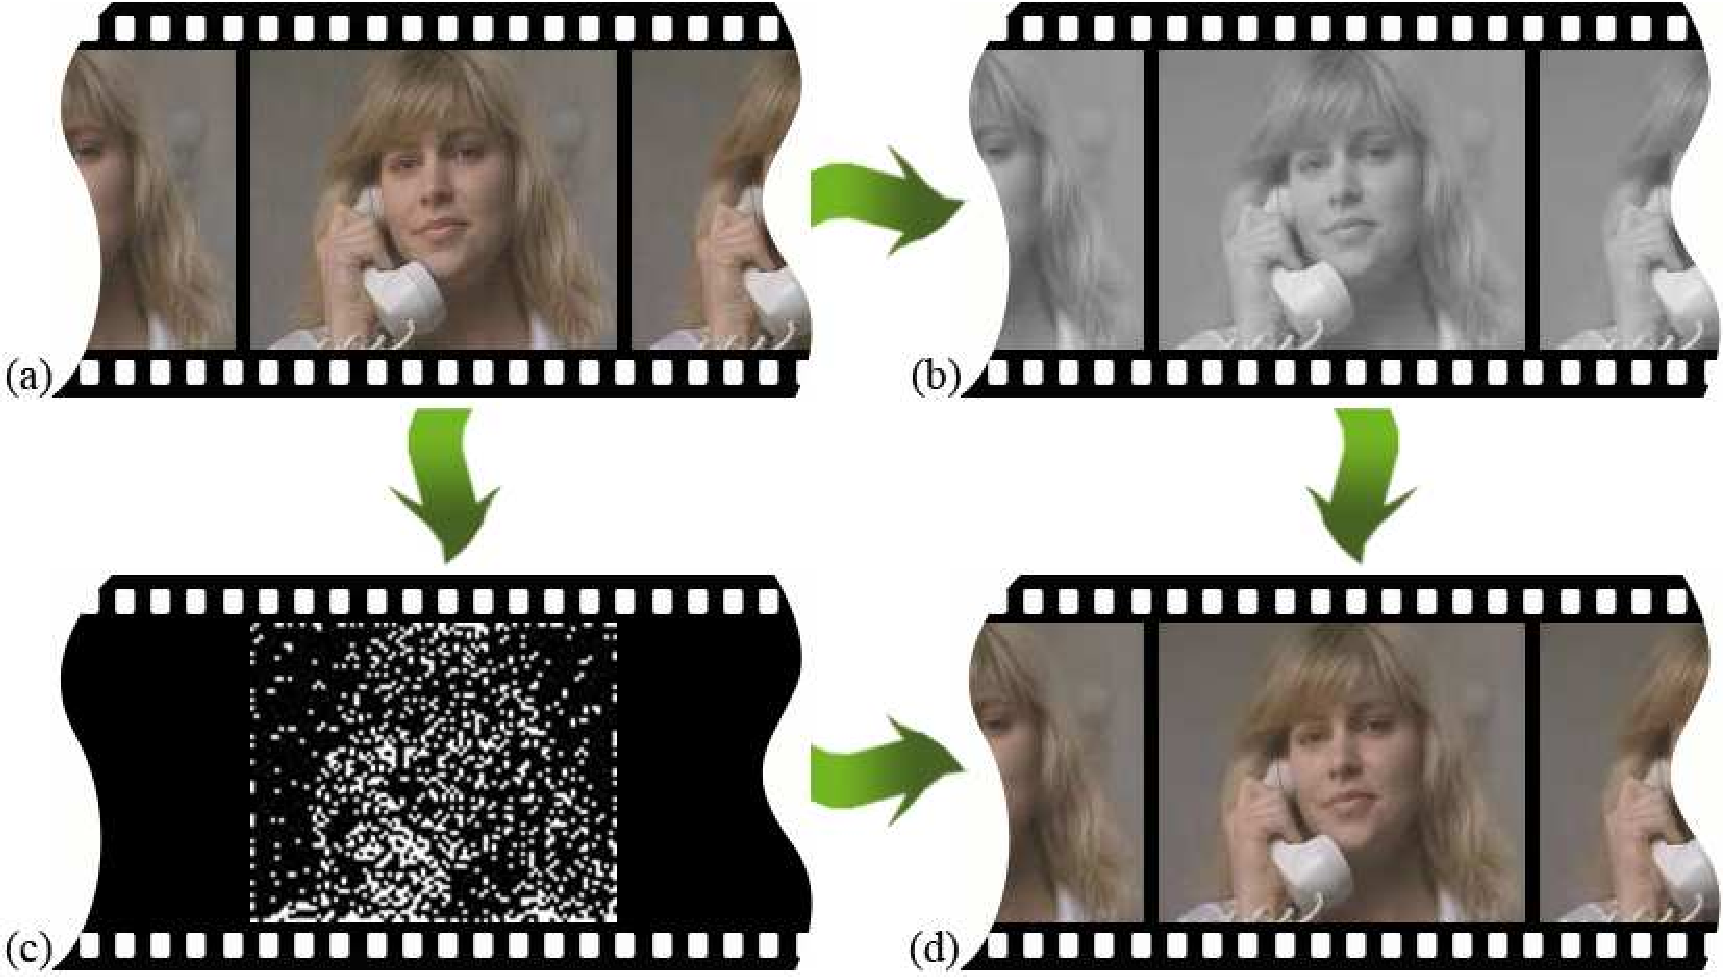
\includegraphics[width=380pt]{images/cycle}}
\caption{\label{fig:cycle}基于学习的视频压缩的例子。 (a) 原始视频帧
(b) 灰度帧 (c) 选取的带有颜色信息的点 (d) 恢复的视频帧}
\end{figure*}

在本文中,我们将从视频压缩这个具体的例子出发,来阐述同时结合时间和空间的正则化
给机器学习问题所带来的性能提升。
视频是一种典型的随着时间轴变化的数据,并且通常在
时间上的变化是比较平滑的,正好是时空正则化的典型应用场景。视频压缩是一项用于缓解
视频存储空间以及传输带宽占用的
关键性技术。视频数据通常包含了许多时间和空间上的冗余信息。相似信息可以通过编码帧内
(空间上的)或帧间(时间上的)差异的方式来进行存储。
典型的压缩方法包括了离散余弦变换、 向量化、分形压缩以及离散小波变换等。

最近 \cite{learning-to-compress-images}
提出了基于机器学习的视频压缩方法。他们提出了和传统的频域转换不同的方式,将原始的带颜色的视频
转化为一个灰度视频,选取一些有代表性的点并存储他们的颜色信息,然后使用灰度视频和带有颜色信息
的点学习出一个统计模型,用于预测其他像素点的颜色值。实验结果表明,在保证图像质量(通过
PSNR
\footnote{http://en.wikipedia.org/wiki/PSNR}进行衡量)的前提下,可以达到不错的压缩效果。

从机器学习的视角来看,这里主要有两个基本的问题。首先是如何选取最有代表性的点,这本质上是一个
主动学习(Active
Learning)的问题。存储灰度视频和选出来的颜色点的信息就是编码的过程。
其次是如何结合选出来的带颜色信息的点和灰度视频来学习一个模型,这在本质上是
一个半监督学习(Semi-supervised
Learning)的问题。用这个模型来恢复原始视频就是解码的过程。在这里有颜色的像素被当作是带标签的
数据,而灰度像素则被当作是无标签的数据。\cite{learning-to-compress-images}
使用了一种非常直接的主动学习的方法:在每一次迭代的时候简单地在预测错误率最高的区域选点。在选
点之后他们使用拉普拉斯正则化的最小二乘法(LapRLS,\cite{Manifold-Regularization-Journal})来
完成半监督学习的问题。他们的方法的最大的不足就是没有任何理论上的依据可以保证使用这种方法选出来
的点可以降低预测的错误率。

在本文中,我们将提出一个针对视频压缩的自主学习和半监督学习的统一框架,并使用时空正则化的方法
对其进行改进以获得性能提升。我们的方法的中心思想是颜色
点的选取和后续的着色过程应该同时进行优化。具体来讲,对于着色的过程,我们假定每个像素的颜色值可以
通过其(时间或空间上的)邻居中灰度值相似的像素的颜色值重新构造出来,并使用正则化的最小二乘法
来学习一个模型;对于选点的过程,我们使用相同的损失函数(loss
function),并使用最小化系数的协方差矩阵的准则来进行选点。然后我们还讨论了如何将自主学习和半监督
学习结合起来应用到视频压缩上面。学习出来的模型不仅用于预测当前的帧,而且还被用于预测后续的相似的
帧,知道 PSNR 分值降低超过了一定的阈值,再重新训练一个模型。图
\ref{fig:cycle} 展示了我们的方法是如何工作的。

论文余下的部分是这样组织的:在第二章中,我们简要地回顾了一下这个领域相关的工作。用于着色的半监督
学习的办法将会在第三章中介绍。第四章介绍如何通过主动学习选取最具代表性的点。然后我们会在第五章中
给出一个用于视频压缩的主动学习和半监督学习的统一框架并运用时空正则化的方法进行改进。实验结果将在
第六章中展示。第七章我们将会进行简要总结并展望后续的工作。

